\chapter{Results}

\section{Carotid Segmentation from TOF-MRA}
As illustrated in Figure~\ref{fig:seg_compare}, the cuboid mask plays a crucial role in carotid segmentation.
Because no ground-truth segmentation is available, results were evaluated by visual inspection.
An example 3D rendering of a segmented ICA is shown in Figure~\ref{fig:carotid_3d}.

\begin{figure}[h]
	\centering
	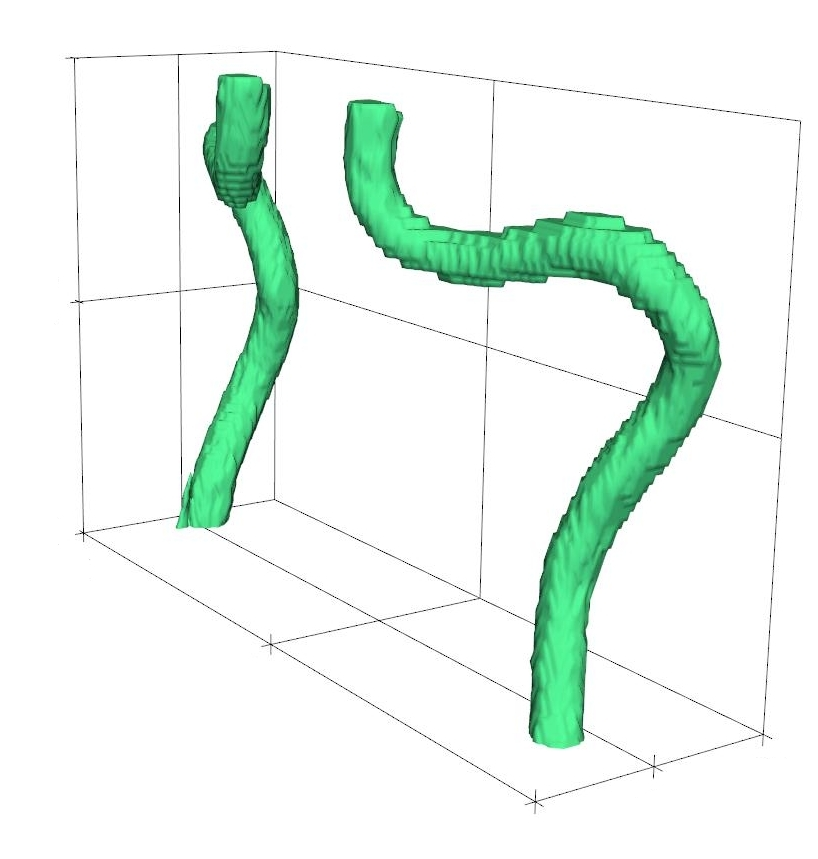
\includegraphics[width=0.3\textwidth]{figures/carotid_3d.jpg}
	\caption{Three-dimensional visualization of the segmented internal carotid arteries.}
	\label{fig:carotid_3d}
\end{figure}

\begin{figure}[h]
	\centering
	\begin{subfigure}{0.45\textwidth}
		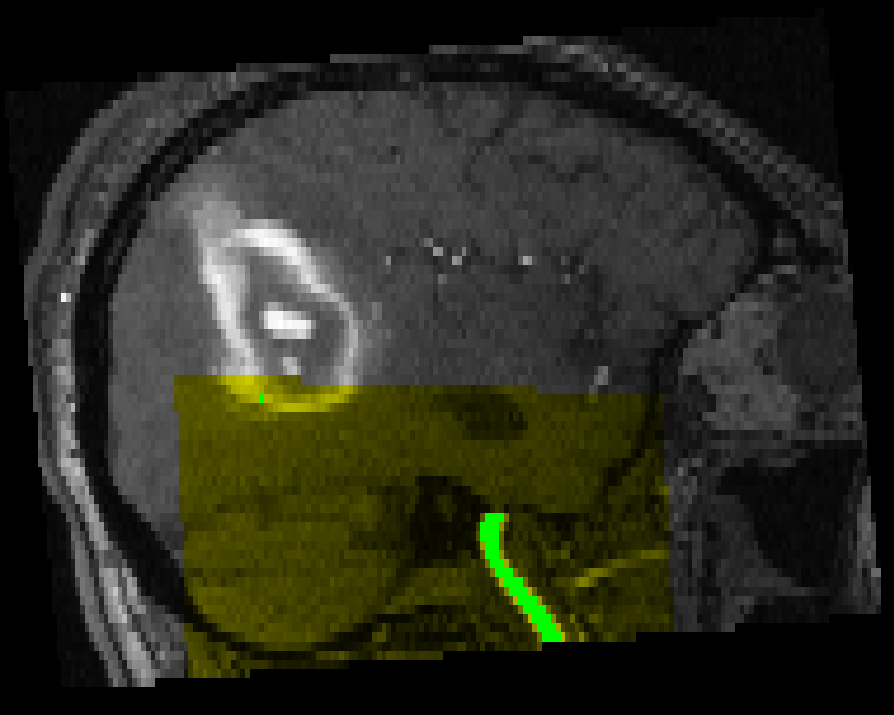
\includegraphics[width=\textwidth]{figures/molgu07704_bbox.png}
		\caption{}
		\label{subfig:seg_bbox}
	\end{subfigure}
	\begin{subfigure}{0.45\textwidth}
		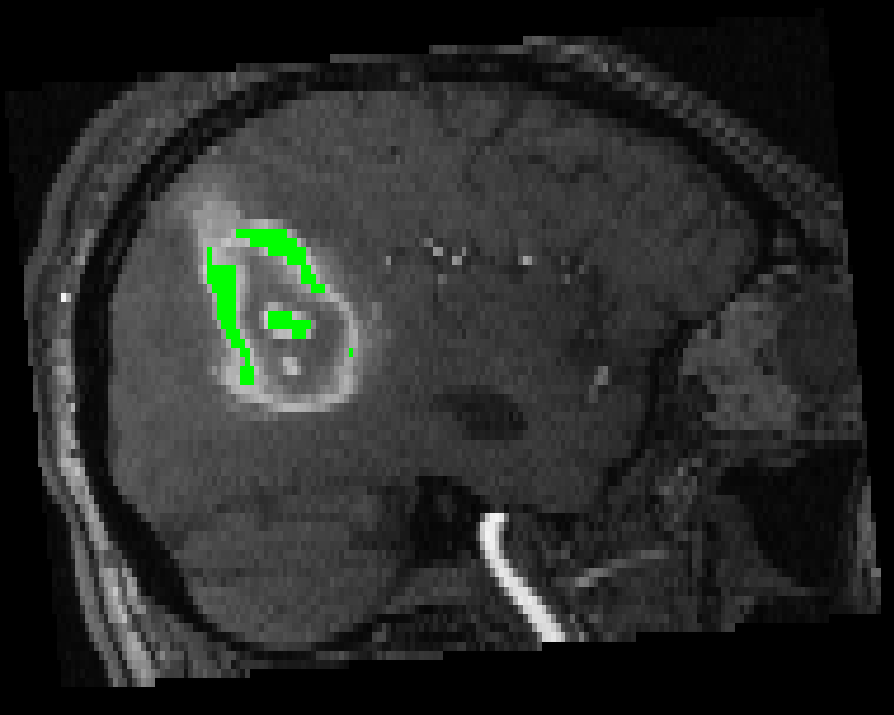
\includegraphics[width=\textwidth]{figures/molgu07704_nobbox.png}
		\caption{}
		\label{subfig:seg_nobbox}
	\end{subfigure}
	\caption{Comparison of carotid segmentation (green) with (a) and without (b) a cuboid mask (yellow).}
	\label{fig:seg_compare}
\end{figure}

\section{Hyperparameter Tuning}
The number of principal components \(p\) was set to 3 based on the cumulative explained-variance curve in Figure~\ref{fig:pca_variance}.
With three components, the cumulative explained variance exceeds 90\%.
To assess the minimal population size needed to build the PCA model in the \fdg\ dataset, the analysis was repeated ten times with different random seeds for \(N\in\{5,10,15,20,30,40,50,60\}\), and median quantification errors were compared.
As shown in Figure~\ref{fig:pca_population}, performance plateaued at \(N=20\), which was therefore adopted.
For the \yohimbine\ dataset, the maximum feasible \(N=6\) was used given the cohort size of seven subjects.

\begin{figure}[h]
	\centering
	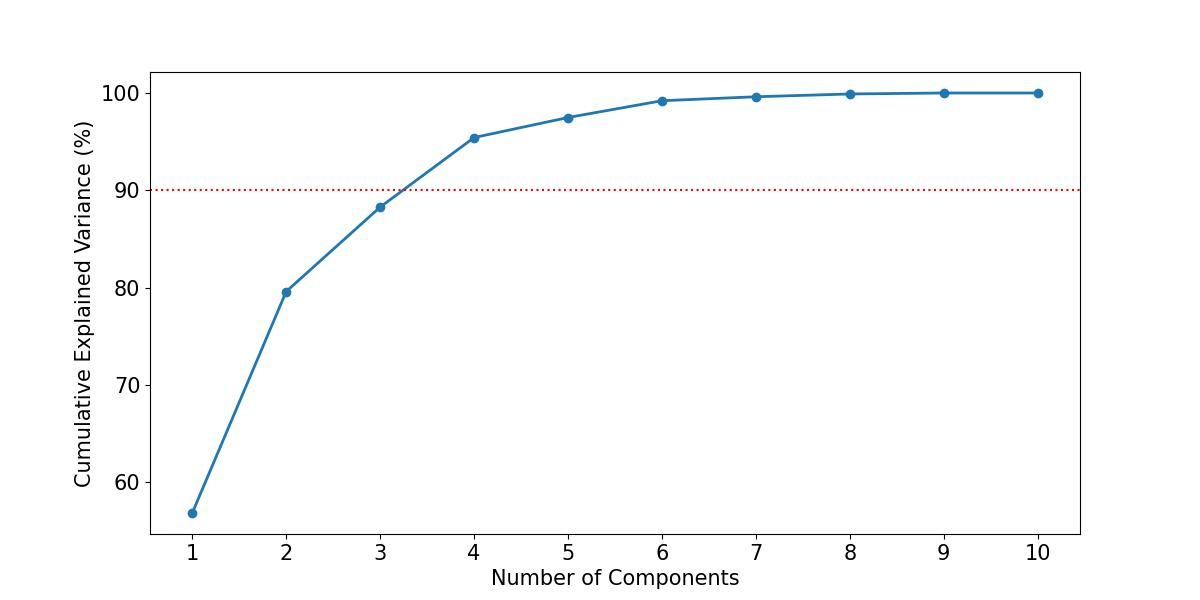
\includegraphics[width=0.8\textwidth]{figures/pca_explained_variance.jpg}
	\caption{Cumulative explained variance as a function of the number of PCA components.}
	\label{fig:pca_variance}
\end{figure}

\begin{figure}[h]
	\centering
	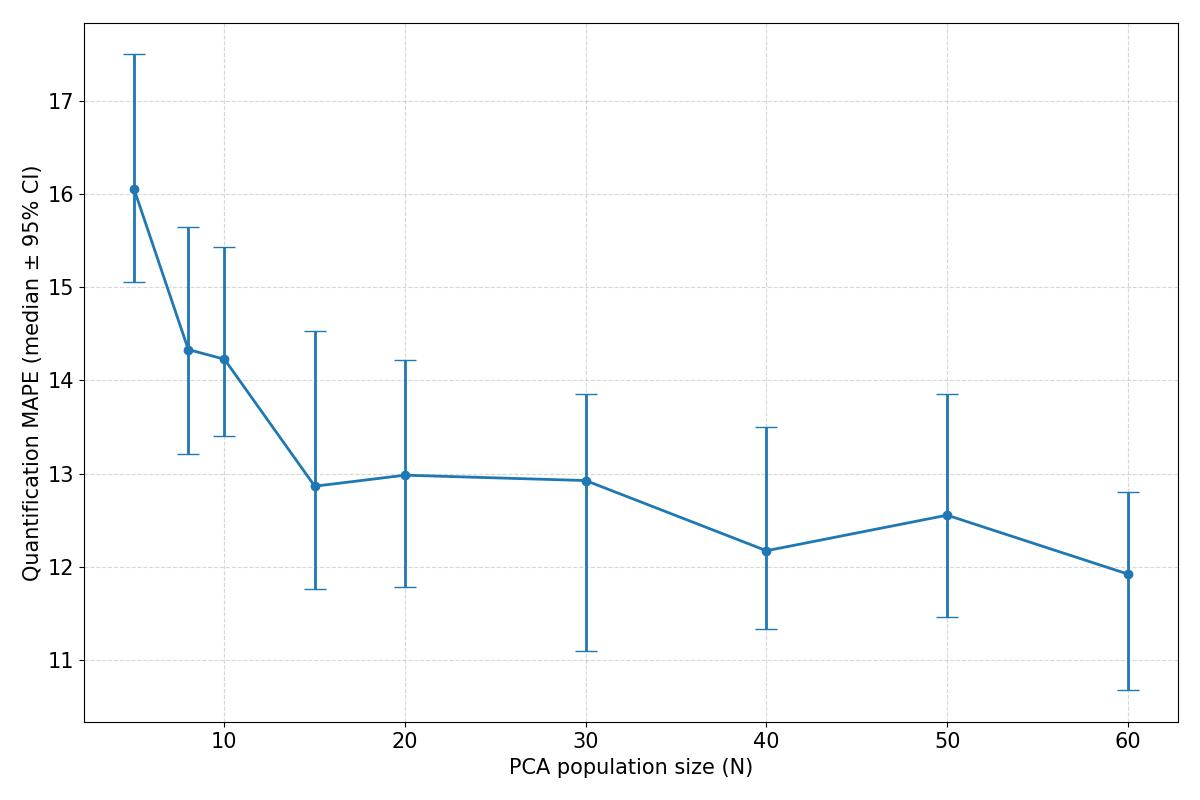
\includegraphics[width=0.7\textwidth]{figures/pca_n_experiment.jpg}
	\caption{Median quantification error (MAPE) with 95\% confidence intervals versus PCA population size.}
	\label{fig:pca_population}
\end{figure}

In classical spectral analysis, the spectral range is chosen according to the isotope half-life (e.g., \(10^{-4}\,\mathrm{s}^{-1}\) to \(1\,\mathrm{s}^{-1}\) for \(^{18}\mathrm{F}\)) and discretized into \(s=100\) or \(s=1000\) fixed decay rates \(\beta\), while amplitudes \(\alpha\) are fitted to the TAC \cite{cunningham1993spectral}.
Peaks in the resulting spectrum correspond to dominant kinetic components of the TAC.
Estimating hundreds of amplitudes with MCMC would be impractical, so a compact basis is preferred in which both decay rates and amplitudes are learned.
To select the basis size, we assumed the background kinetics could be approximated by the impulse response of either a 1TCM or a 2TCM, which entail one or two exponential basis functions, respectively.
With two basis functions, the sampler frequently converged to nearly identical decay rates or pushed one rate to infinity, indicating a negligible contribution.
Accordingly, a single exponential basis function was used for both datasets.
As discussed in Section~\ref{sec:bgtm_modelling}, the PCA weights were assigned the prior \(\theta_i\sim\mathcal{N}(0,1)\).
The spectral parameters were given weakly informative uniform priors \(\alpha,\beta\sim\mathcal{U}(10^{-5},10^{-2})\) due to the lack of stronger prior knowledge.

Each Markov chain was run for 230{,}000 iterations with a 30{,}000-iteration burn-in to ensure convergence.

\section{Simulation}\label{sec:results_simulation}
Of the 59 \fdg\ subjects, 24 were excluded because large tumors or post-surgical skull openings caused the tissue-classification algorithm to fail.
The remaining 35 subjects were used to build numerical phantoms and to generate TACs for the simulation protocol.
The PET-SORTEO platform generated realistic PET in sinogram format based on these protocols.
Sinograms were reconstructed with the same software and settings as the experimental data to ensure consistency.

The simulations were intended for quality control of the pipeline rather than replication of individual scans, and comparisons to real data were used only as sanity checks.
Figure~\ref{fig:sim_compare_imgs} shows sagittal slices from the second and last frames for a representative subject, including the real PET, the simulation input, and the simulation output.
Less detail is visible in the neck region because we did not model the full arterial tree, the venous system, or glands.
The early frame (top row) roughly coincides with the AIF peak and the activity in the ICA is clearly visible.
In the late frame, when the tissues reach steady state, the brain activity seems realistic, and we see an adequate contrast between regions such as WM and GM.

Figure~\ref{fig:sim_tac_compare} compares a partial-volume–corrected TAC from the simulation output with its simulation input.
As expected, there are small differences due to noise in larger regions such as GM and the cerebellum, and there is a clear bias in the ICA because it is strongly affected by partial-volume effects.

\begin{figure}[h]
	\centering
	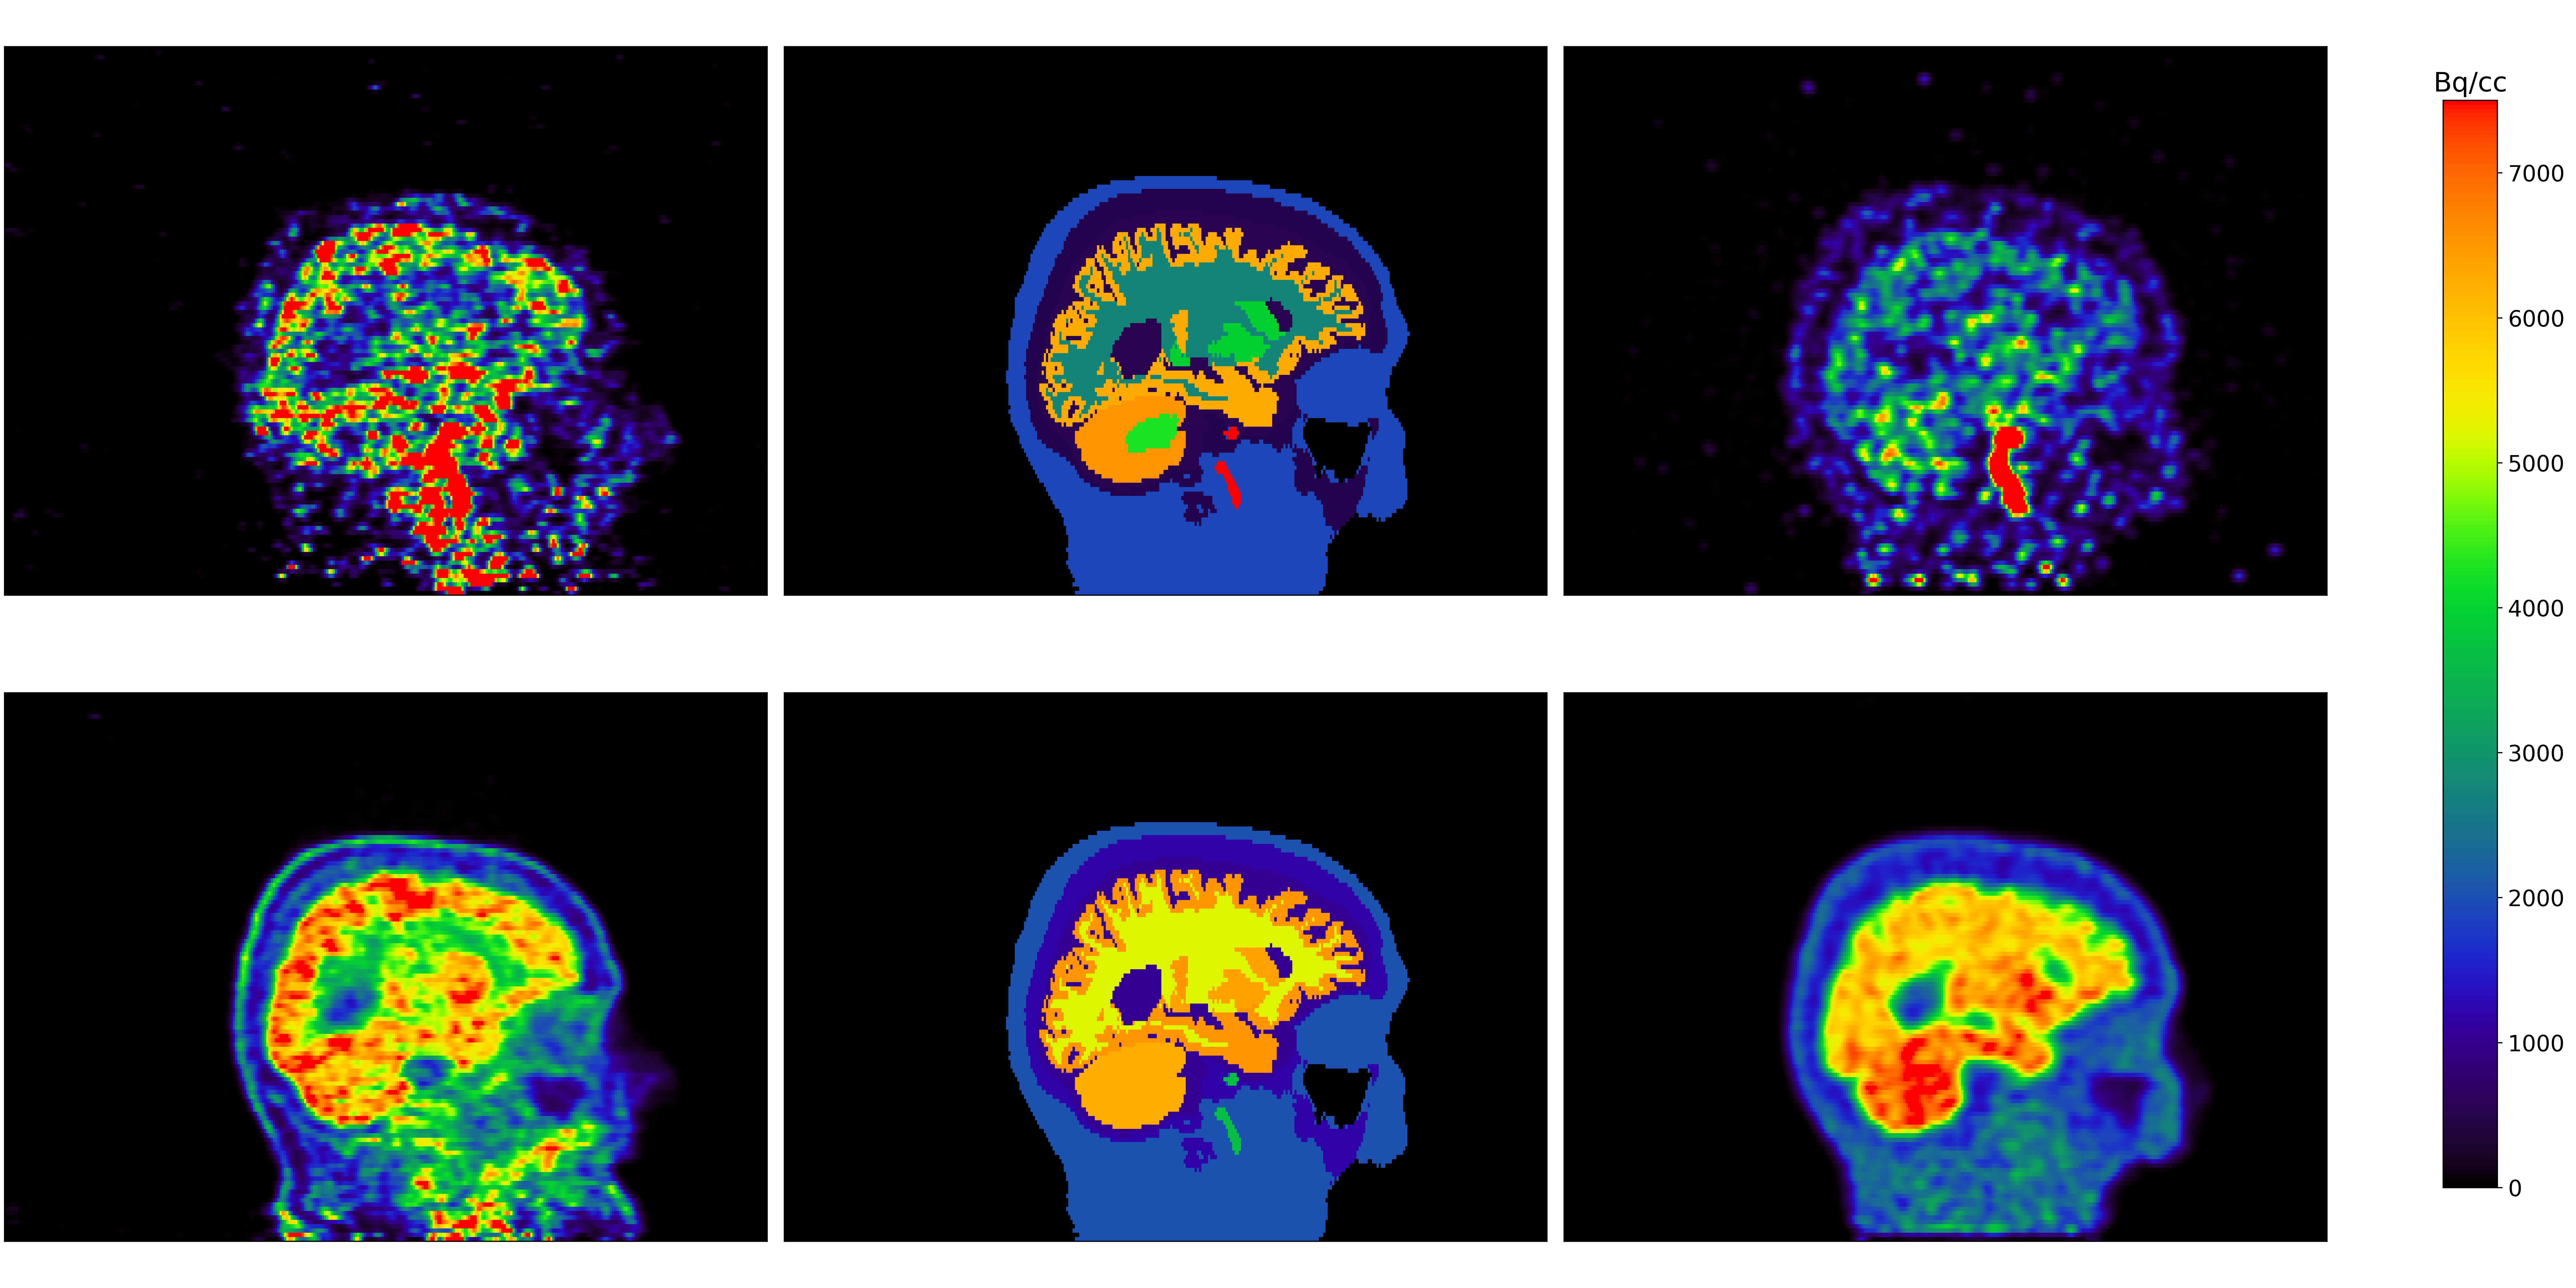
\includegraphics[width=\textwidth]{figures/sim_compare.jpg}
	\caption{Sagittal slices from the second frame (top) and last frame (bottom) for real PET (left), simulation input (middle), and simulation output (right)}
	\label{fig:sim_compare_imgs}
\end{figure}

\begin{figure}[h]
	\centering
	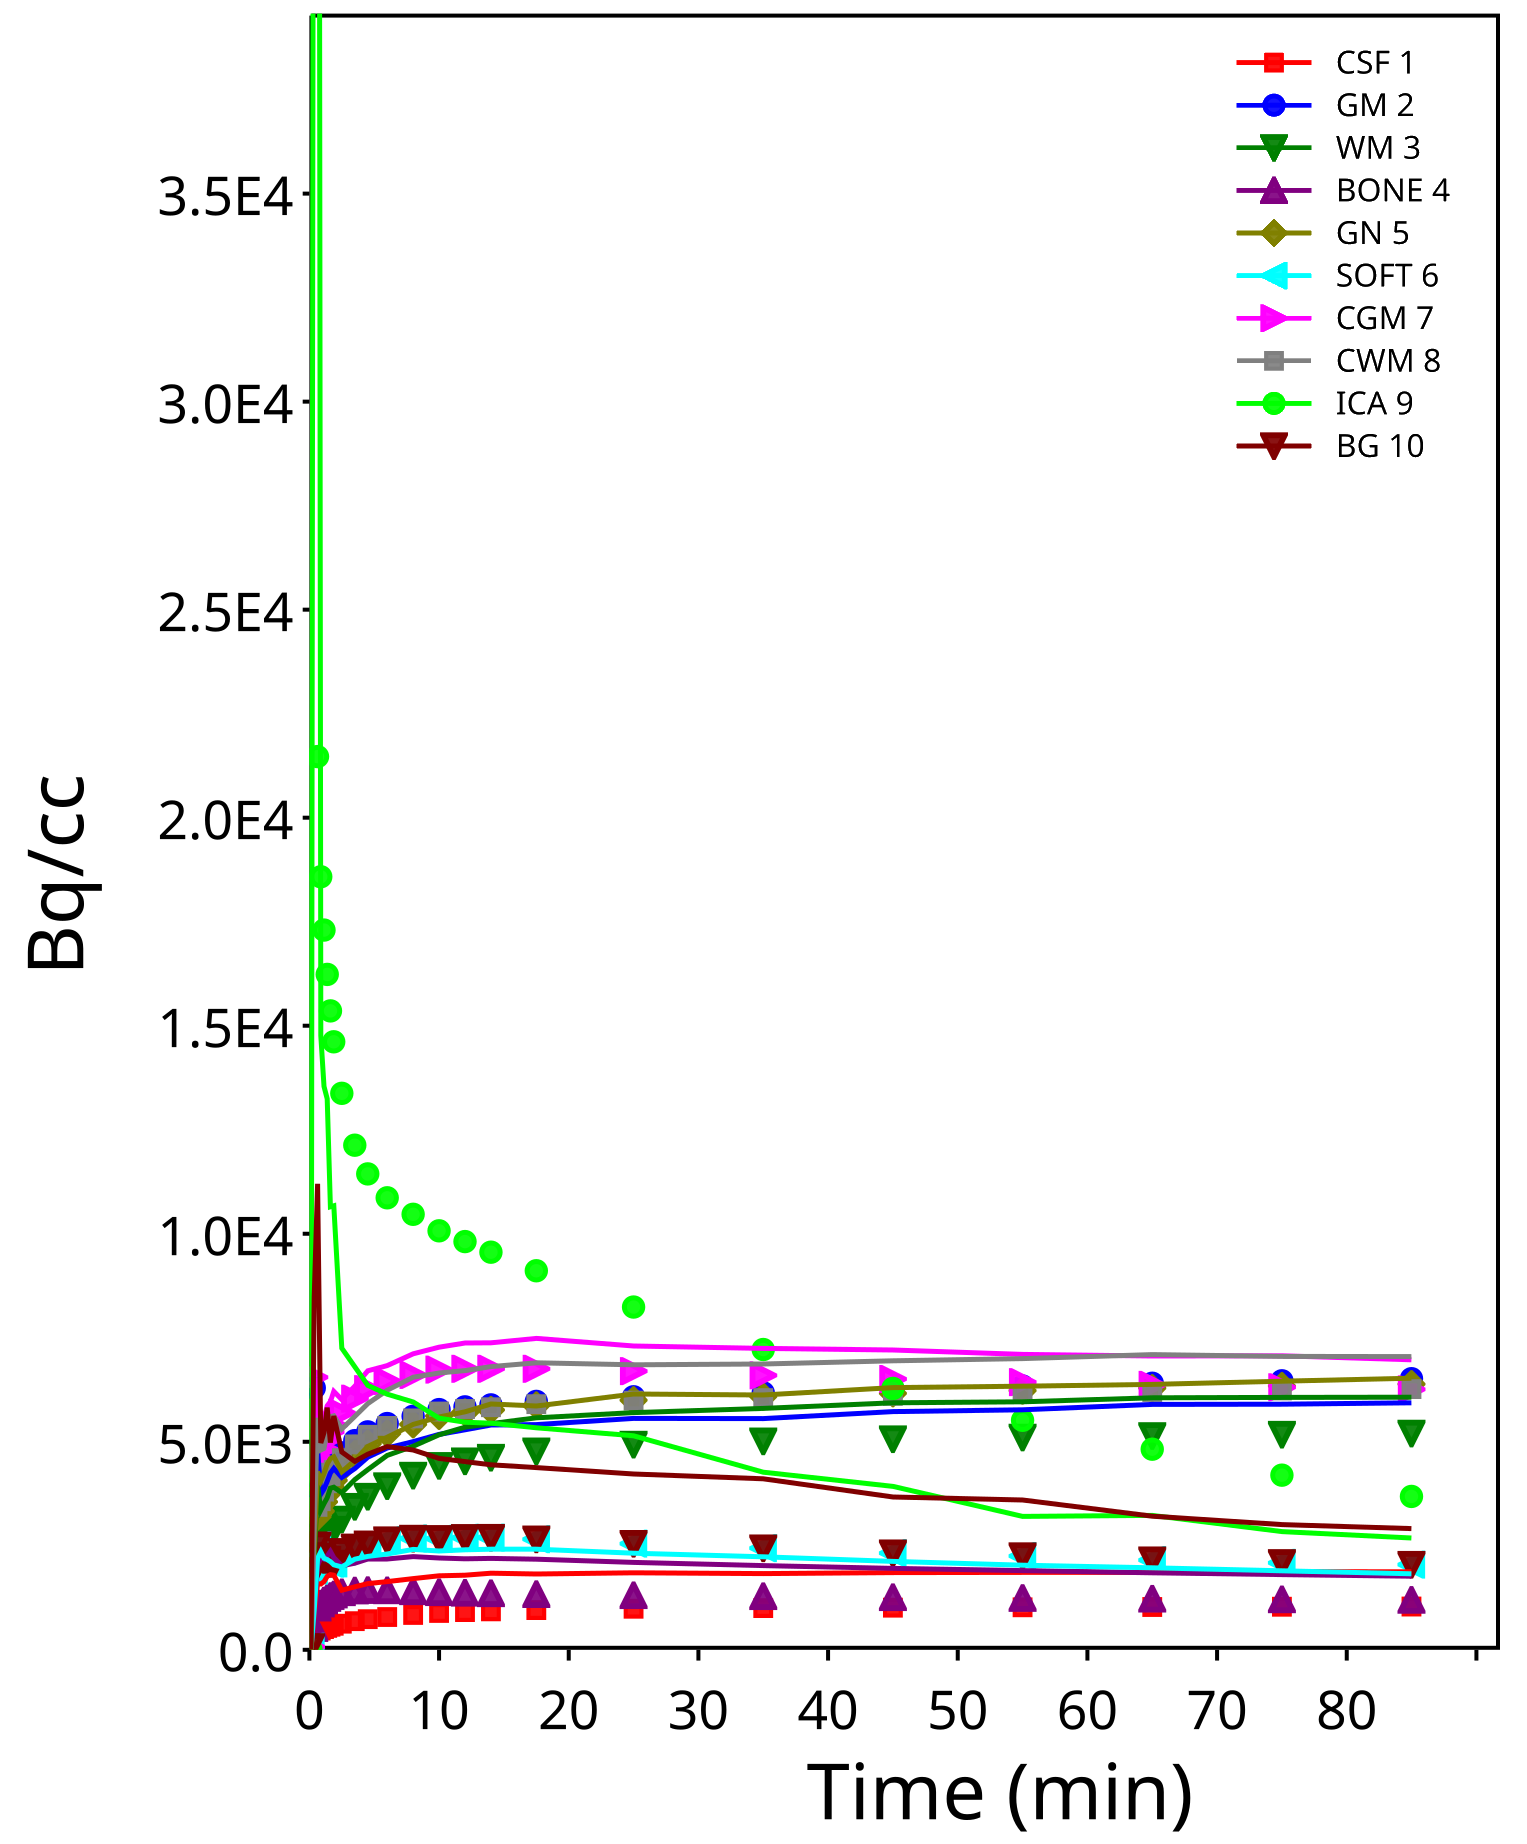
\includegraphics[width=0.4\textwidth]{figures/sim_tac.png}
	\caption{TAC Comparison of the simulation input (dots) and the partial-volume–corrected output (lines) of an example subject}
	\label{fig:sim_tac_compare}
\end{figure}

\section{IDIF}
Because BGTM builds on GTM and incorporates a population AIF prior, performance was compared with GTM-derived IDIF and with a PBIF defined as the mean AIF used in the PCA (\(\mu_{IF}\)).

\subsection{\fdg\ Dataset}
The reported statistics correspond to the experiment yielding the median validation performance from the fine-tuning stage.
Figure~\ref{fig:fdg_ifs} illustrates best- and worst-case subjects.
In the better-performing subject, BGTM outperforms GTM and PBIF (\(\mrglu\) MAPE of 1.2\% versus 26\% and 1.6\%, respectively), whereas in the poorer-performing subject BGTM underperforms relative to GTM and PBIF (\(\mrglu\) MAPE of 36\% versus 2.2\% and 4.75\%, respectively).

\begin{figure}[h]
	\centering
	\begin{subfigure}[b]{0.322\textwidth}
		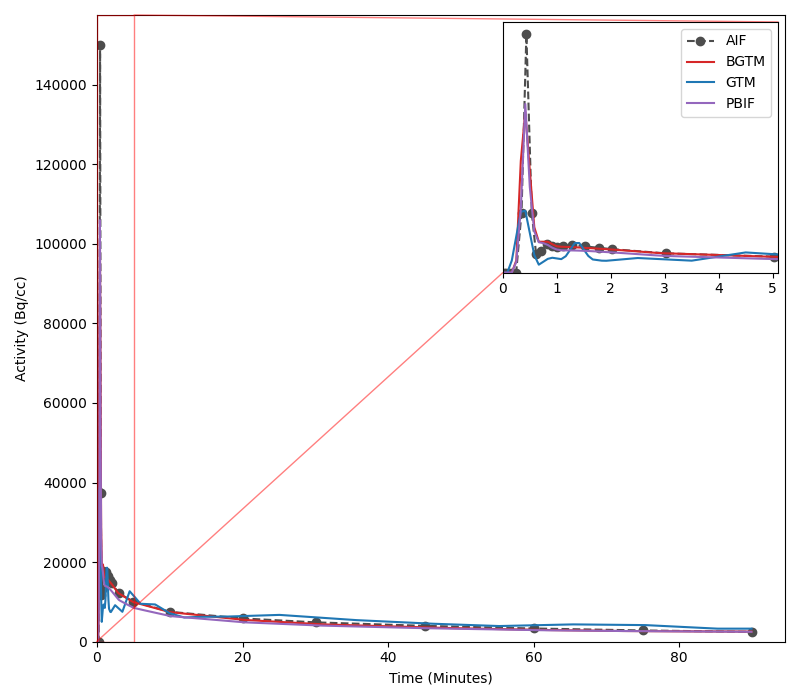
\includegraphics[width=\textwidth]{figures/PM10845_1_infunc.png}
		\caption{}
	\end{subfigure}
	\begin{subfigure}[b]{0.322\textwidth}
		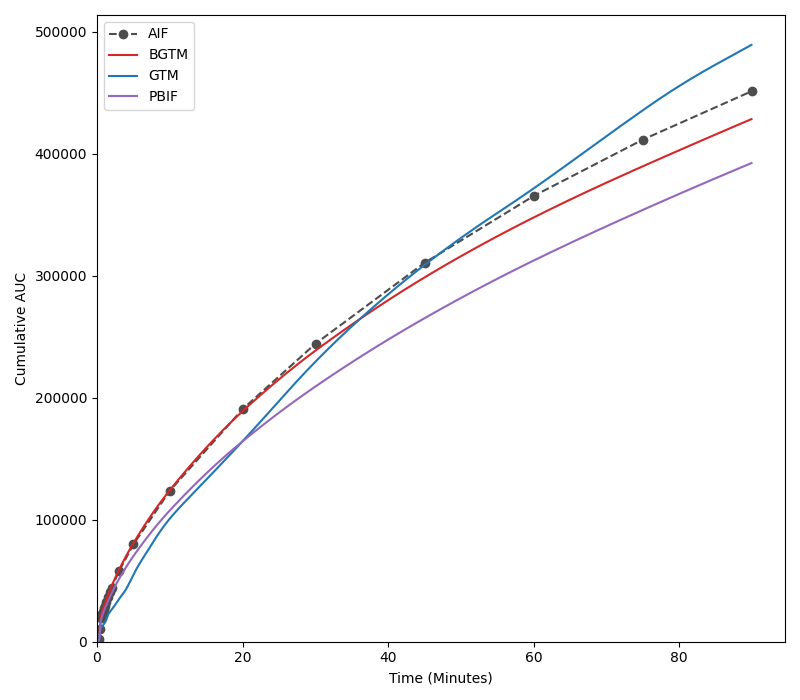
\includegraphics[width=\textwidth]{figures/PM10845_1_cauc.png}
		\caption{}
	\end{subfigure}
	\begin{subfigure}[b]{0.322\textwidth}
		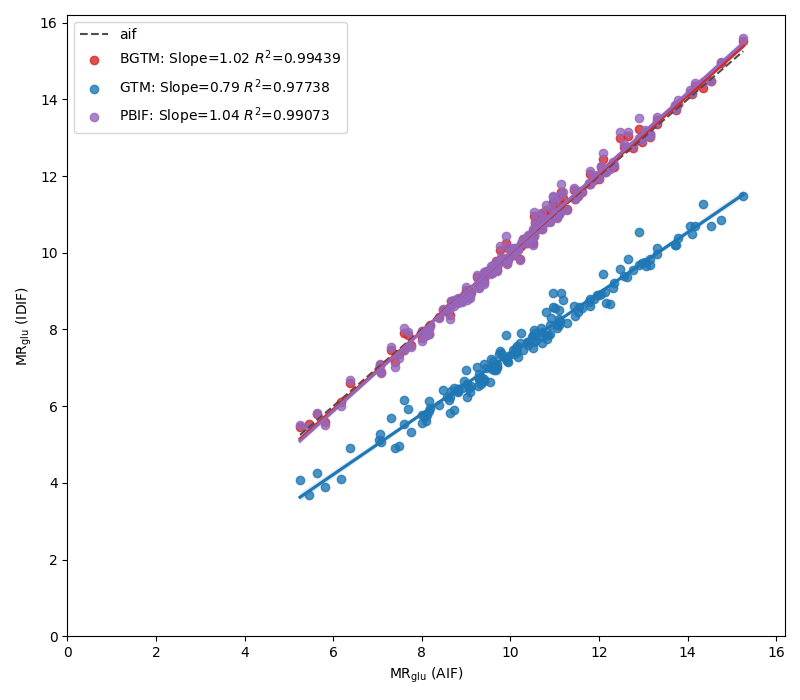
\includegraphics[width=\textwidth]{figures/PM10845_1_patlak_mrglu.png}
		\caption{}
	\end{subfigure}
	\begin{subfigure}[b]{0.322\textwidth}
		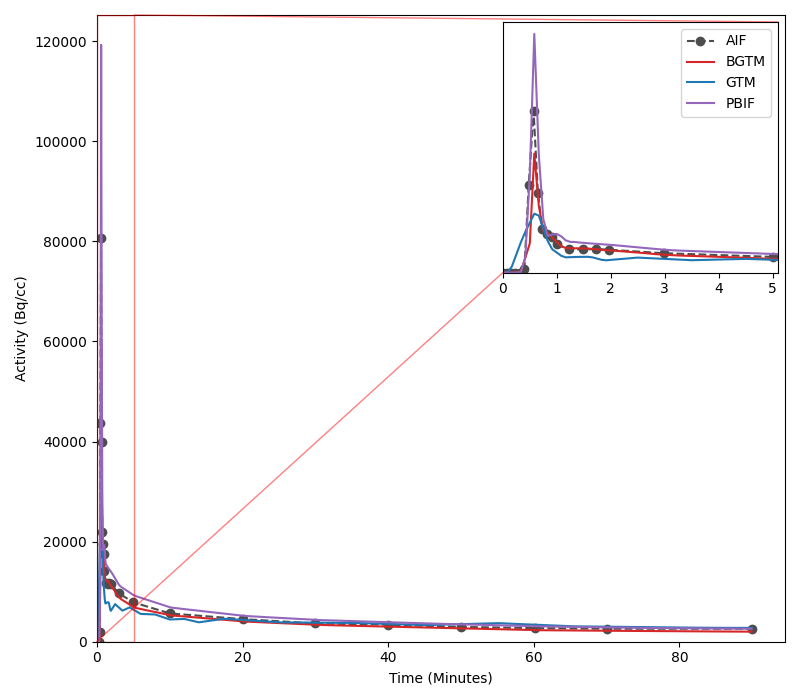
\includegraphics[width=\textwidth]{figures/COUJE07810_1_infunc.png}
		\caption{}
	\end{subfigure}
	\begin{subfigure}[b]{0.322\textwidth}
		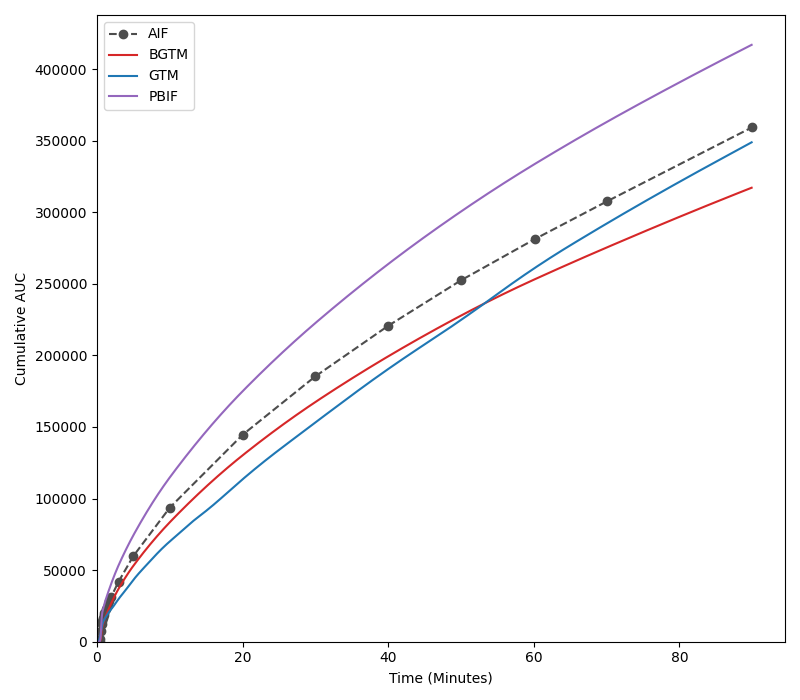
\includegraphics[width=\textwidth]{figures/COUJE07810_1_cauc.png}
		\caption{}
	\end{subfigure}
	\begin{subfigure}[b]{0.322\textwidth}
		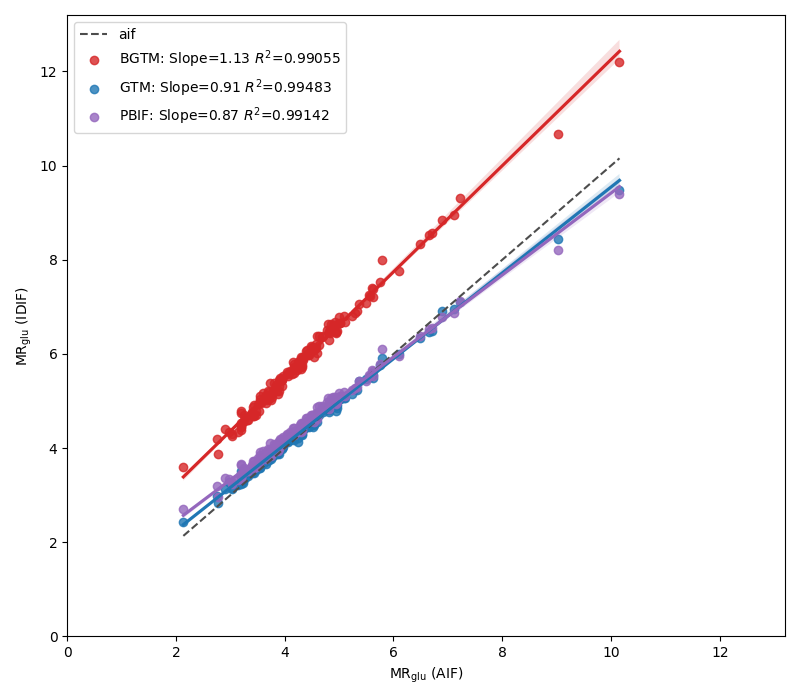
\includegraphics[width=\textwidth]{figures/COUJE07810_1_patlak_mrglu.png}
		\caption{}
	\end{subfigure}
	\caption{Comparison of the IFs (a,d), cumulative AUC curves (b,e), and \(\mrglu\) regression lines (c,f) for one better-performing (top) and one poorer-performing (bottom) subject in the \fdg\ dataset.}
	\label{fig:fdg_ifs}
\end{figure}

The average cAUC MAE across subjects was 13{,}024 for BGTM and 15{,}709 and 14{,}630 for GTM and PBIF, respectively (Figure~\ref{subfig:fdg_cauc_boxplot}).
In quantification, BGTM achieved lower errors than GTM and PBIF.
Specifically, the average \(\mrglu\) MAPE was 13\%, 24\%, and 17\% for BGTM, GTM, and PBIF, respectively (Figure~\ref{subfig:fdg_mape_boxplot}), and the average \(\mrglu\) MAE was 1.04, 1.98, and 1.40.
The MAPE for the coefficient of determination \((R^2)\) and the regression slope \((S)\) was 1.75\% and 11.2\% for BGTM, versus 4.1\% and 17\% for GTM and 1.5\% and 15.75\% for PBIF, respectively.

\begin{figure}[h]
	\centering
	\begin{subfigure}[b]{0.45\textwidth}
		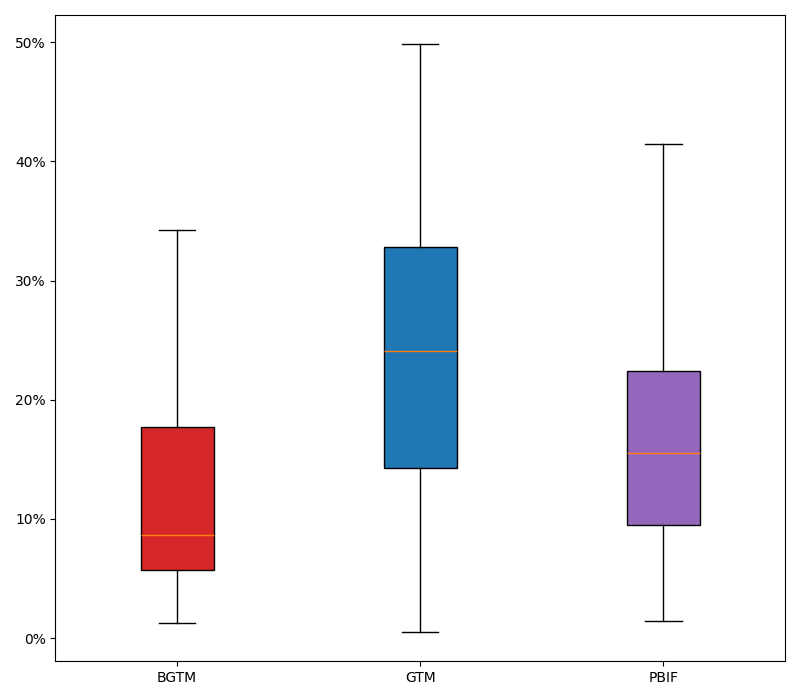
\includegraphics[width=\textwidth]{figures/fdg_quantification_patlak_mape_boxplot.png}
		\caption{\(\mrglu\) MAPE boxplot.}
		\label{subfig:fdg_mape_boxplot}
	\end{subfigure}
	\begin{subfigure}[b]{0.45\textwidth}
		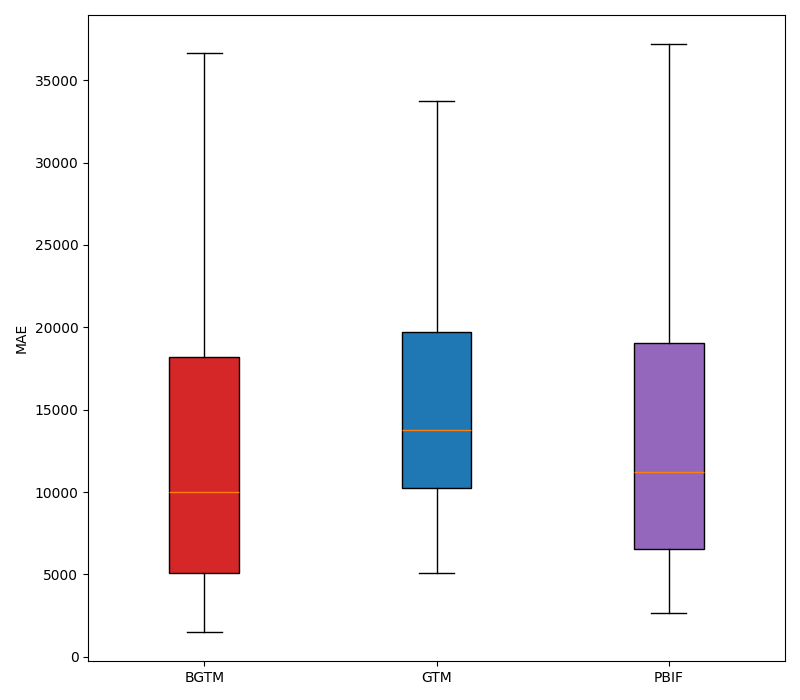
\includegraphics[width=\textwidth]{figures/fdg_curve_mae_boxplot.png}
		\caption{cAUC MAE boxplot.}
		\label{subfig:fdg_cauc_boxplot}
	\end{subfigure}
	\caption{Boxplots of curve and quantification errors for the \fdg\ dataset.}
	\label{fig:fdg_boxplots}
\end{figure}

Paired t-tests were used to compare BGTM with GTM and PBIF on quantification metrics (Table~\ref{tab:metrics_all_fdg}).
Relative to GTM, BGTM showed significantly lower \(\mrglu\) MAE (\(t=-5.934, p=1.754\times 10^{-7}\)), \(\mrglu\) MAPE (\(t=-5.459,\,p=1.042\times 10^{-6}\)), \(R^2\) absolute percentage error (APE) (\(t=-2.762,\,p=7.677\times 10^{-3}\)), and slope APE (\(t=-4.030,\,p=1.644\times 10^{-4}\)).
Relative to PBIF, BGTM also yielded significantly lower \(\mrglu\) MAE (\(t=-2.974,\,p=4.275\times 10^{-3}\)), \(\mrglu\) MAPE (\(t=-2.415,\,p=1.890\times 10^{-2}\)), and slope APE (\(t=-3.036,\,p=3.583\times 10^{-3}\)), while the difference in \(R^2\) APE was not significant (\(t=1.680,\,p=9.832\times 10^{-2}\)).

\subsection{\yohimbine\ Dataset}
Performance on the \yohimbine\ dataset was lower than on \fdg.
Figure~\ref{fig:yoh_ifs} compares best- and worst-performing subjects.
Across subjects, the average cAUC MAE was 55{,}499 for BGTM and 96{,}362 and 37{,}613 for GTM and PBIF, respectively (Figure~\ref{subfig:yoh_cauc_boxplot}).
By Logan analysis, the average \(V_T\) MAPE was 75.9\%, 166.5\%, and 29.5\% for BGTM, GTM, and PBIF, respectively (Figure~\ref{subfig:yoh_mape_boxplot}).

\begin{figure}[h]
	\centering
	\begin{subfigure}[b]{0.322\textwidth}
		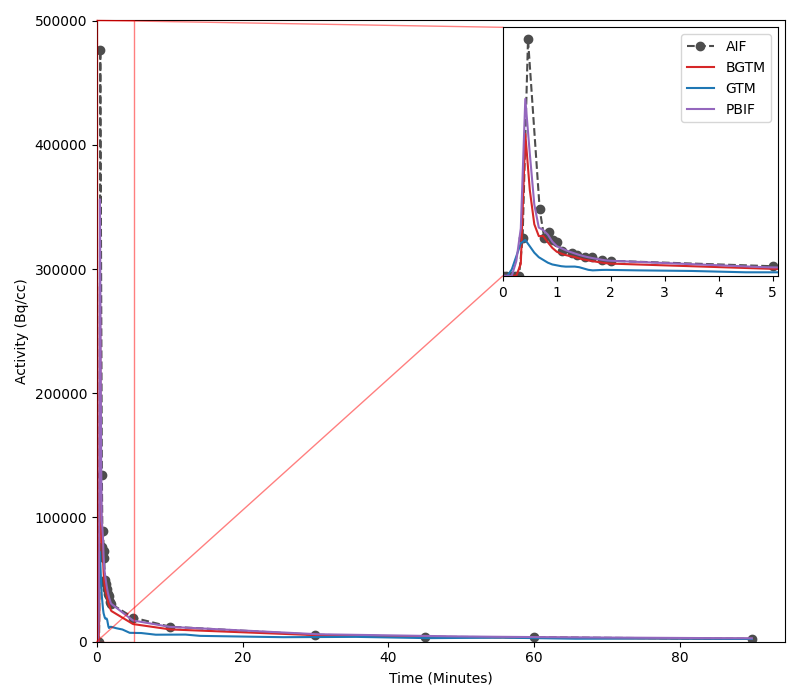
\includegraphics[width=\textwidth]{figures/LUCAU08056_TEST_infunc.png}
		\caption{}
	\end{subfigure}
	\begin{subfigure}[b]{0.322\textwidth}
		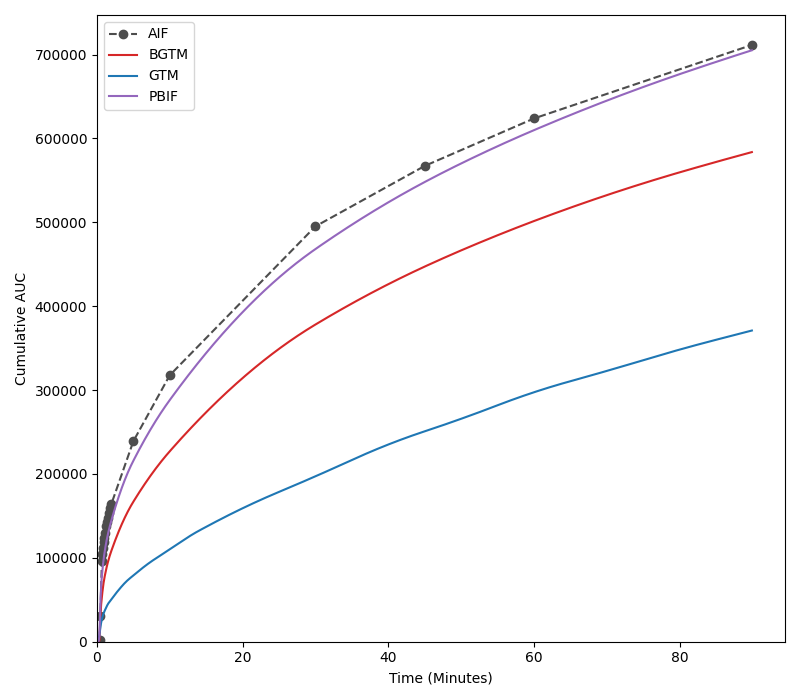
\includegraphics[width=\textwidth]{figures/LUCAU08056_TEST_cauc.png}
		\caption{}
	\end{subfigure}
	\begin{subfigure}[b]{0.322\textwidth}
		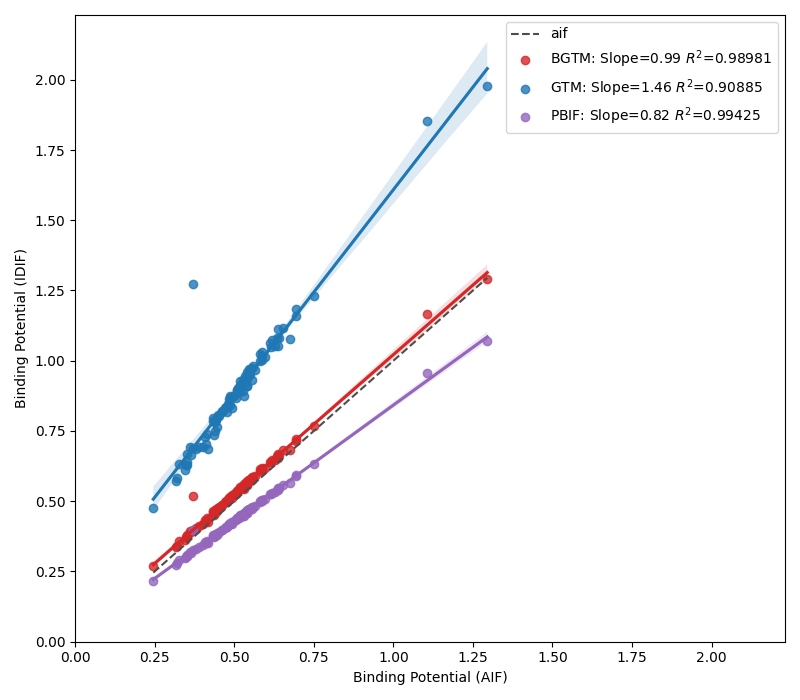
\includegraphics[width=\textwidth]{figures/LUCAU08056_TEST_logan_bp.png}
		\caption{}
	\end{subfigure}
	\begin{subfigure}[b]{0.322\textwidth}
		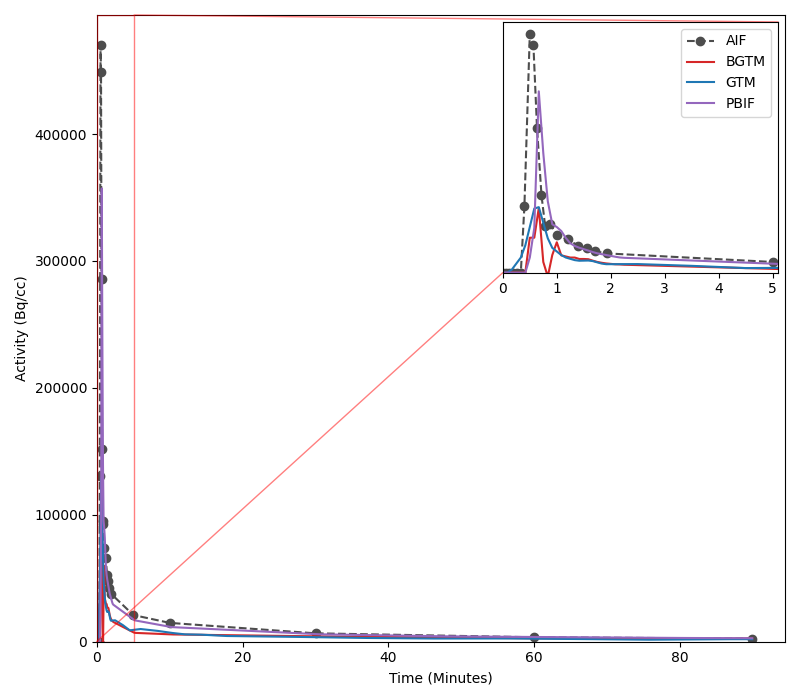
\includegraphics[width=\textwidth]{figures/GOIAX07977_TEST_infunc.png}
		\caption{}
	\end{subfigure}
	\begin{subfigure}[b]{0.322\textwidth}
		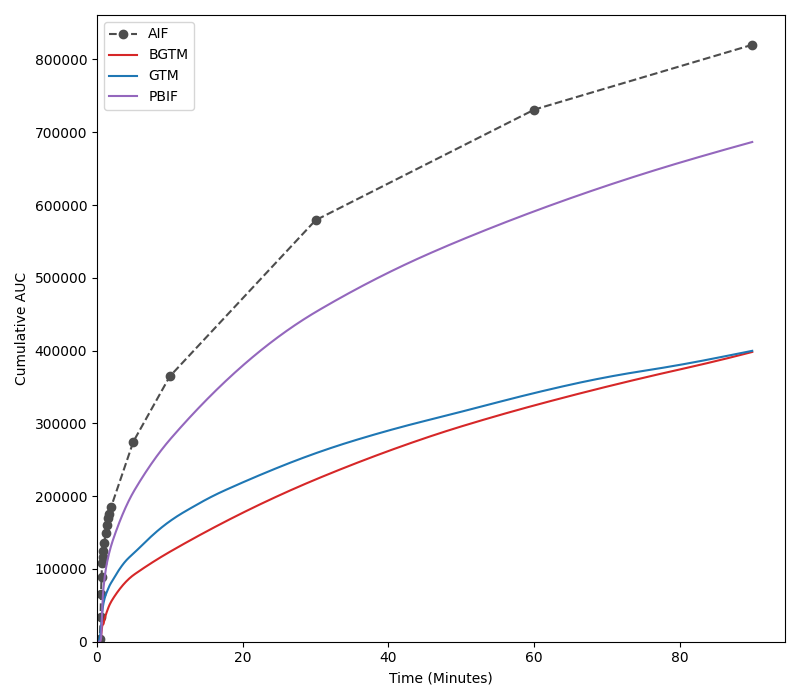
\includegraphics[width=\textwidth]{figures/GOIAX07977_TEST_cauc.png}
		\caption{}
	\end{subfigure}
	\begin{subfigure}[b]{0.322\textwidth}
		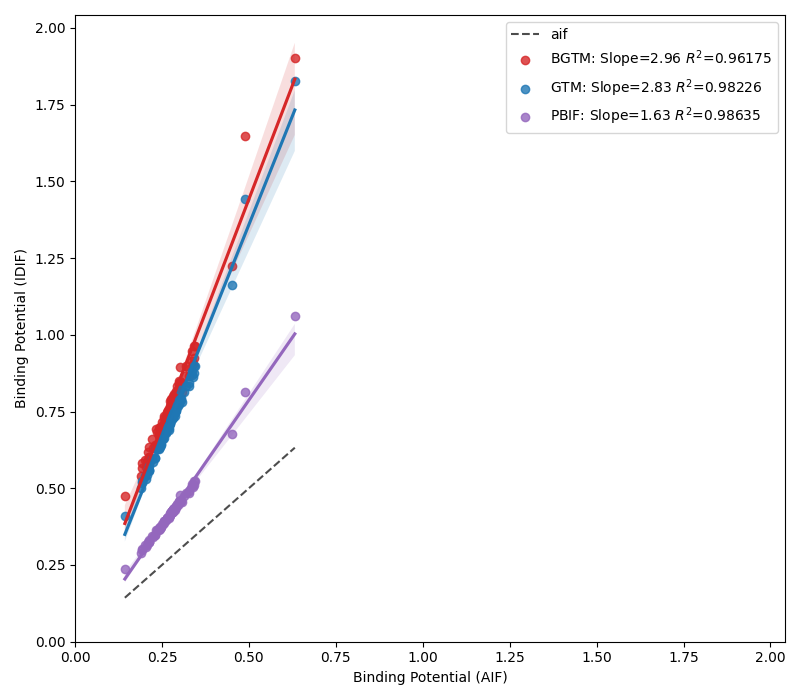
\includegraphics[width=\textwidth]{figures/GOIAX07977_TEST_logan_bp.png}
		\caption{}
	\end{subfigure}
	\caption{Comparison of the IFs (a,d), cumulative AUC curves (b,e), and \(V_T\) regression lines (c,f) for one better-performing (top) and one poorer-performing (bottom) subject in the \yohimbine\ dataset.}
	\label{fig:yoh_ifs}
\end{figure}

\begin{figure}[h]
	\centering
	\begin{subfigure}[b]{0.45\textwidth}
		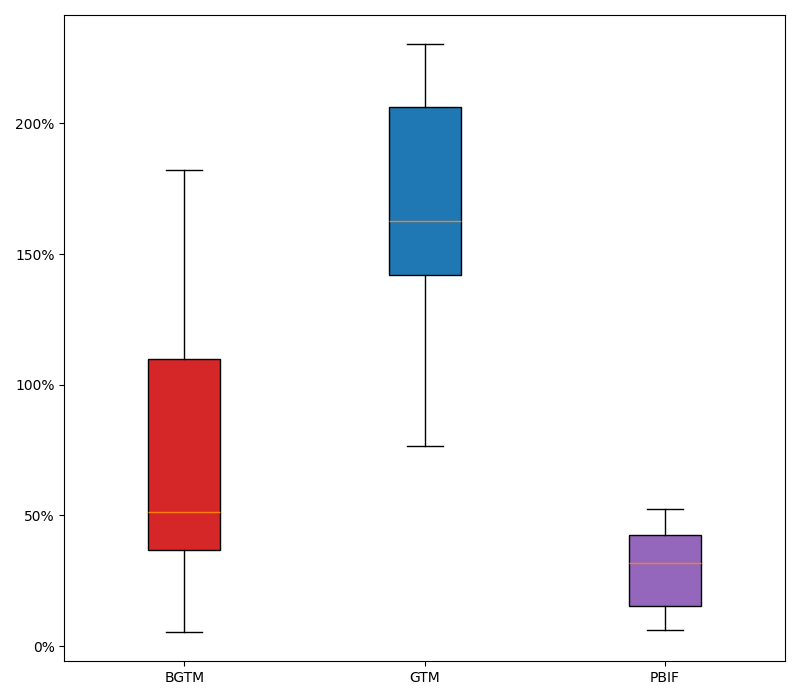
\includegraphics[width=\textwidth]{figures/yoh_quantification_logan_mape_boxplot.png}
		\caption{\(V_T\) MAPE boxplot.}
		\label{subfig:yoh_mape_boxplot}
	\end{subfigure}
	\begin{subfigure}[b]{0.45\textwidth}
		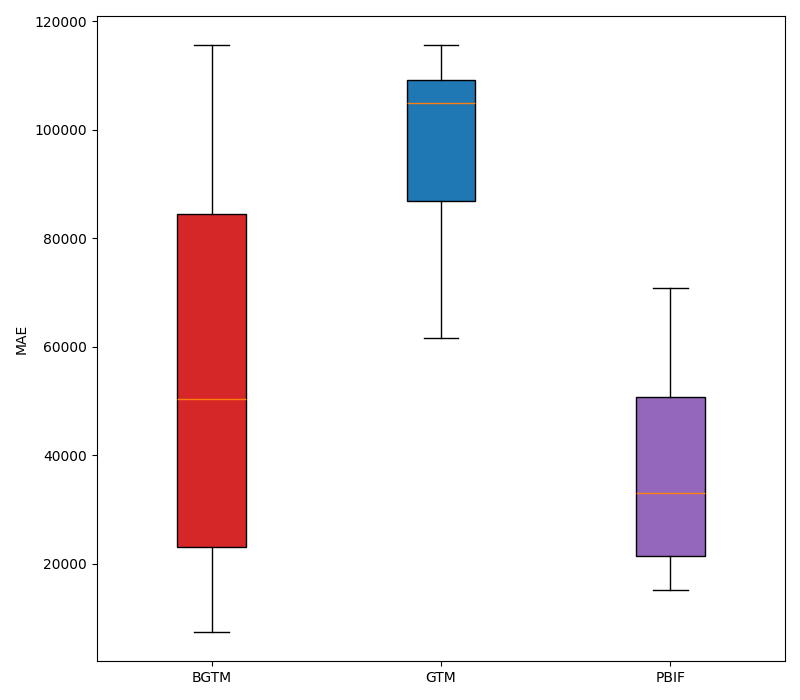
\includegraphics[width=\textwidth]{figures/yoh_curve_mae_boxplot.png}
		\caption{cAUC MAE boxplot.}
		\label{subfig:yoh_cauc_boxplot}
	\end{subfigure}
	\caption{Boxplots of curve and quantification errors for the \yohimbine\ dataset.}
	\label{fig:yoh_boxplots}
\end{figure}

\subsection{Simulated Dataset}
As a quality-control check on the simulations, the Direct IDIF (no PVC) from the experimental data was compared with the Direct IDIF from the simulated data.
The simulated dataset showed a higher cAUC MAE than the experimental dataset (85{,}138 versus 34{,}929) and a higher AUC APE (46\% versus 22\%).
Figure~\ref{fig:sim_temporal_err} shows the temporal error for one subject, where the simulated Direct IDIF underestimates activity relative to the experimental Direct IDIF.

This underestimation propagates to other IDIF methods and increases bias.
Figure~\ref{fig:sim_ifs} shows best- and worst-case subjects.
BGTM provided only a slight improvement in cAUC MAE relative to GTM (53{,}997 versus 57{,}991), and it performed worse than PBIF, which achieved an average cAUC MAE of 23{,}072 (Figure~\ref{subfig:sim_cauc_boxplot}).
In absolute quantification, BGTM underperformed both comparators, with an average \(\mrglu\) MAPE of 48\% versus 35.6\% for GTM and 18.5\% for PBIF.
Paired t-tests showed no improvement over GTM for cAUC MAE (\(t=-1.353,\,p=0.185\)) and statistically worse performance than PBIF for cAUC MAE (\(t=9.013,\,p=1.56\times10^{-10}\)), RMSE (\(t=8.805,\,p=2.73\times10^{-10}\)), and AUC APE (\(t=8.317,\,p=1.04\times10^{-9}\)).


\begin{figure}[h]
	\centering
	\begin{subfigure}[b]{0.322\textwidth}
		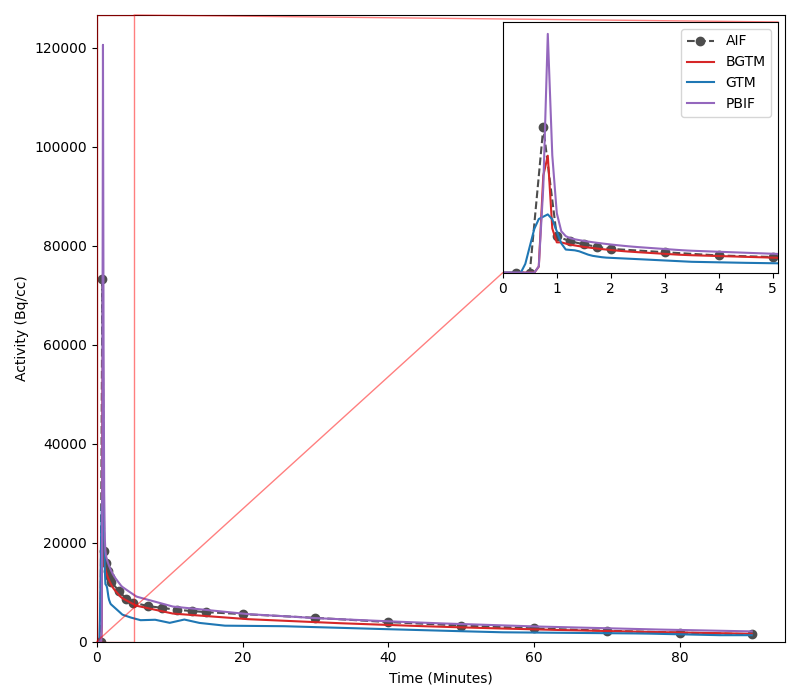
\includegraphics[width=\textwidth]{figures/sim_CHAAB07833_1_infunc.png}
		\caption{}
	\end{subfigure}
	\begin{subfigure}[b]{0.322\textwidth}
		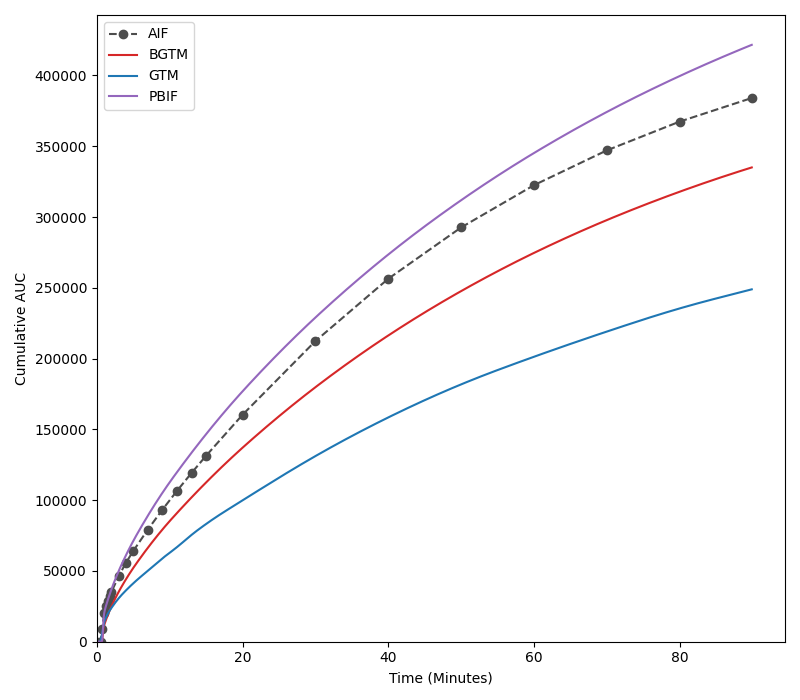
\includegraphics[width=\textwidth]{figures/sim_CHAAB07833_1_cauc.png}
		\caption{}
	\end{subfigure}
	\begin{subfigure}[b]{0.322\textwidth}
		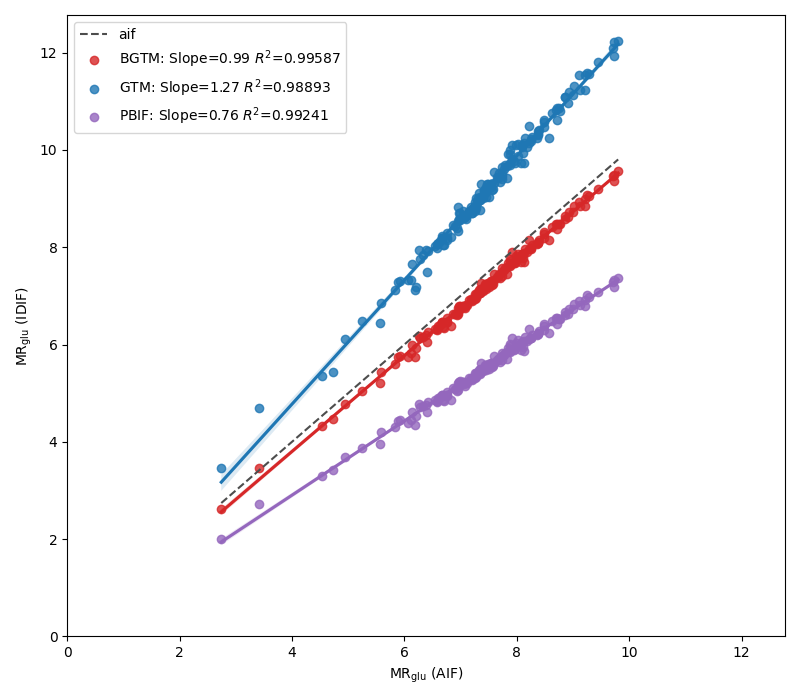
\includegraphics[width=\textwidth]{figures/sim_CHAAB07833_1_patlak_mrglu.png}
		\caption{}
	\end{subfigure}
	\begin{subfigure}[b]{0.322\textwidth}
		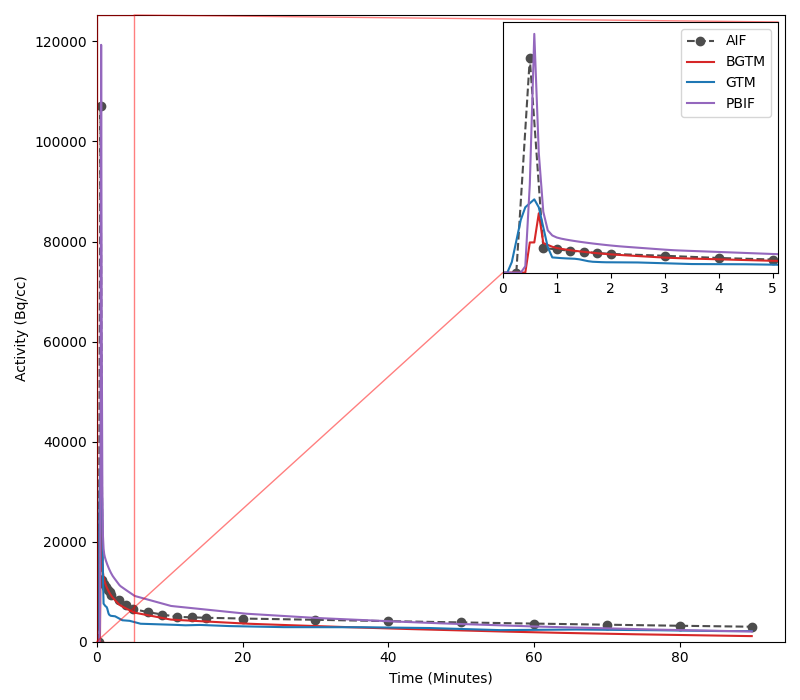
\includegraphics[width=\textwidth]{figures/sim_AJ10923_1_infunc.png}
		\caption{}
	\end{subfigure}
	\begin{subfigure}[b]{0.322\textwidth}
		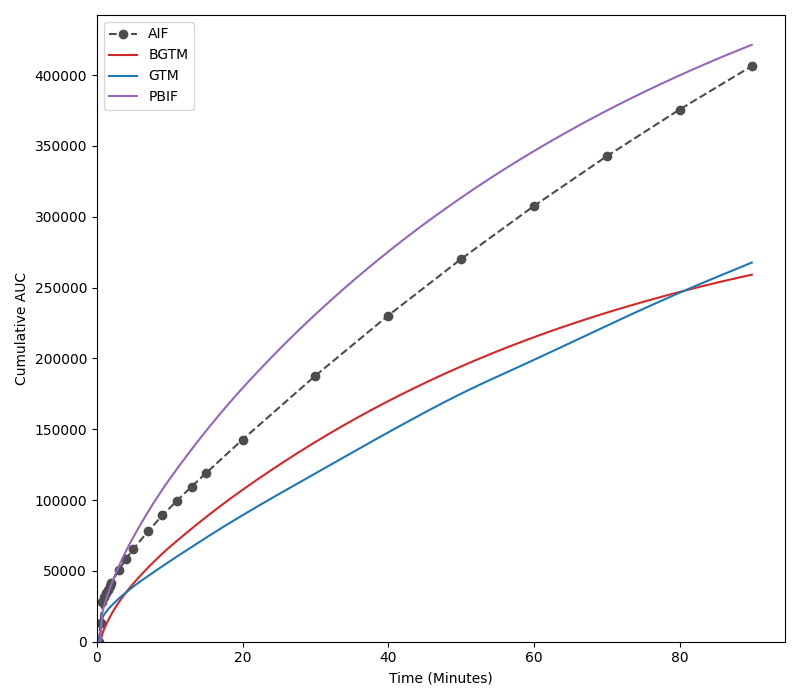
\includegraphics[width=\textwidth]{figures/sim_AJ10923_1_cauc.png}
		\caption{}
	\end{subfigure}
	\begin{subfigure}[b]{0.322\textwidth}
		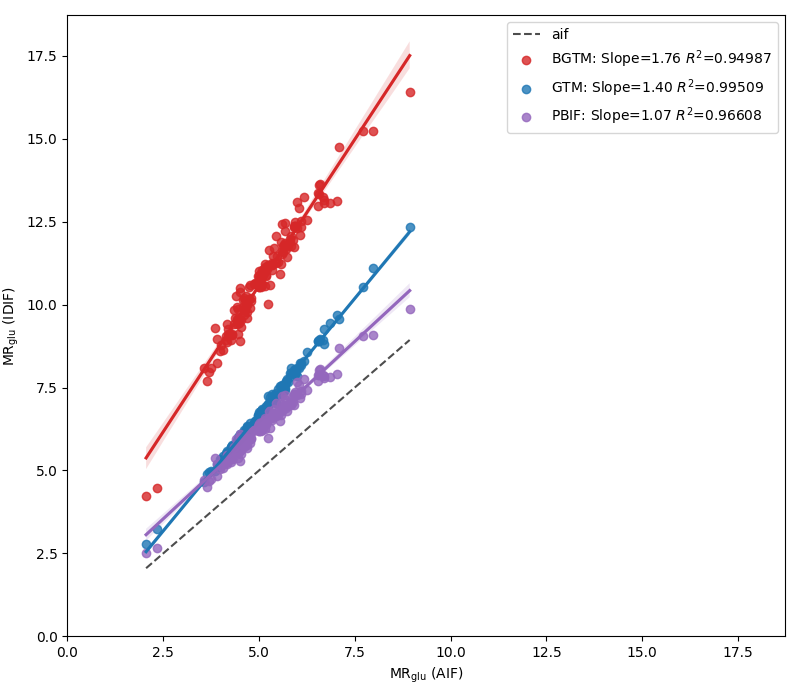
\includegraphics[width=\textwidth]{figures/sim_AJ10923_1_patlak_mrglu.png}
		\caption{}
	\end{subfigure}
	\caption{Comparison of the IFs (a,d), cumulative AUC curves (b,e), and \(\mrglu\) regression lines (c,f) for one better-performing (top) and one poorer-performing (bottom) simulated subject.}
	\label{fig:sim_ifs}
\end{figure}

\begin{figure}[h]
	\centering
	\begin{subfigure}[b]{0.45\textwidth}
		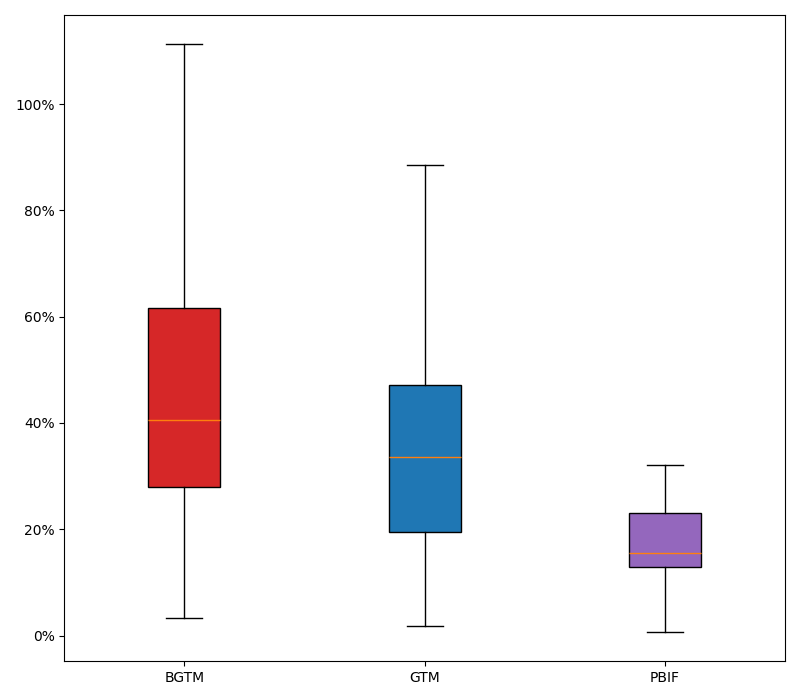
\includegraphics[width=\textwidth]{figures/sim_quantification_patlak_mape_boxplot.png}
		\caption{\(\mrglu\) MAPE boxplot.}
		\label{subfig:sim_mape_boxplot}
	\end{subfigure}
	\begin{subfigure}[b]{0.45\textwidth}
		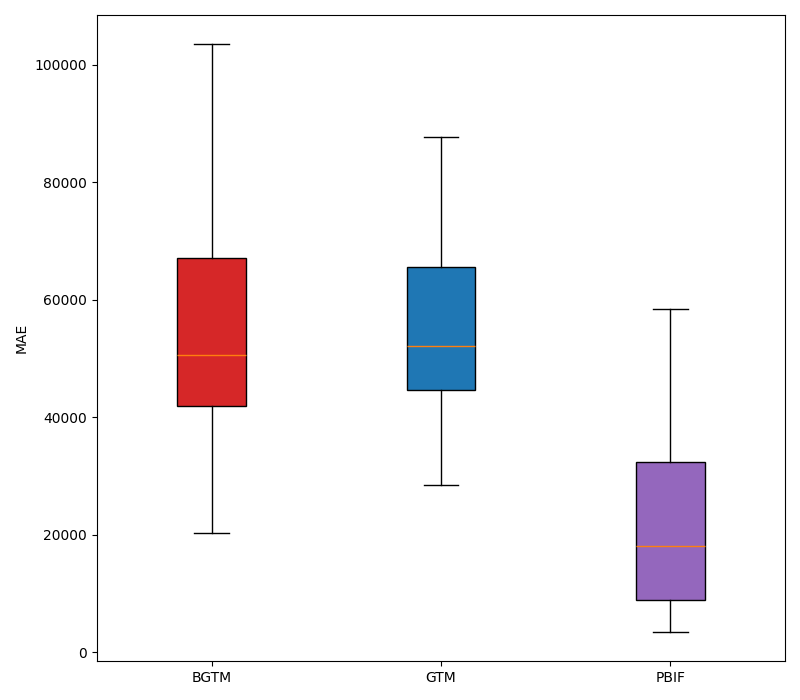
\includegraphics[width=\textwidth]{figures/sim_curve_mae_boxplot.png}
		\caption{cAUC MAE boxplot.}
		\label{subfig:sim_cauc_boxplot}
	\end{subfigure}
	\caption{Boxplots of curve and quantification errors for the simulated dataset.}
	\label{fig:sim_boxplots}
\end{figure}

\begin{figure}[h]
	\centering
	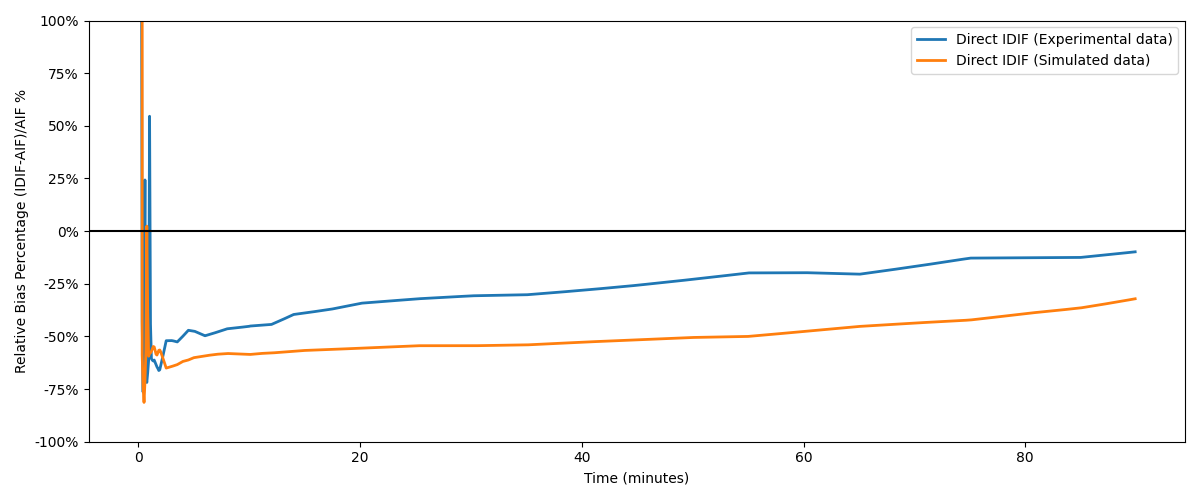
\includegraphics[width=\textwidth]{figures/GM12051_temporal_error.png}
	\caption{Relative temporal bias (\%) of Direct IDIF in one experimental subject versus its simulated counterpart.}
	\label{fig:sim_temporal_err}
\end{figure}


\begin{sidewaystable}[b]
	\centering
	\small
	\setlength{\tabcolsep}{10pt}
	\caption*{\fdg\ Dataset}
	\begin{tabular}{l|cc|cc|cc|cc|cc}
		\toprule
		\multirow{2}{*}{\textbf{Metric}} & \multicolumn{2}{c|}{\textbf{BGTM}} & \multicolumn{2}{c|}{\textbf{GTM}} & \multicolumn{2}{c|}{\textbf{PBIF}} & \multicolumn{2}{c|}{\textbf{BGTM vs GTM}} & \multicolumn{2}{c}{\textbf{BGTM vs PBIF}}                                                                                                                  \\
		\cmidrule(lr){2-3} \cmidrule(lr){4-5} \cmidrule(lr){6-7} \cmidrule(lr){8-9} \cmidrule(lr){10-11}
		                                 & \(\mu\)                            & \(\sigma\)                        & \(\mu\)                            & \(\sigma\)                                & \(\mu\)                                   & \(\sigma\) & \(t\)      & \(p\)                              & \(t\)      & \(p\)                              \\
		\midrule
		IF cAUC MAE                      & 13{,}024                           & 10{,}410                          & 15{,}709                           & 7{,}884                                   & 14{,}630                                  & 10{,}268   & \(-2.388\) & \(2.023\times 10^{-2}\) \sym{*}    & \(-1.278\) & \(2.065\times 10^{-1}\)            \\
		IF cAUC RMSE                     & 20{,}293                           & 16{,}078                          & 23{,}380                           & 11{,}979                                  & 23{,}334                                  & 16{,}803   & \(-1.907\) & \(6.151\times 10^{-2}\) \sym{\dag} & \(-1.439\) & \(1.555\times 10^{-1}\)            \\
		IF AUC APE (\%)                  & 11.93                              & 10.76                             & 11.57                              & 11.50                                     & 14.34                                     & 11.08      & \(0.297\)  & \(7.674\times 10^{-1}\)            & \(-1.862\) & \(6.767\times 10^{-2}\) \sym{\dag} \\
		\midrule
		\(\mrglu\) MAPE (\%)             & 13.19                              & 10.57                             & 24.36                              & 13.68                                     & 17.17                                     & 12.41      & \(-5.459\) & \(1.042\times 10^{-6}\) \sym{***}  & \(-2.415\) & \(1.890\times 10^{-2}\) \sym{*}    \\
		\(\mrglu\) MAE                   & 1.04                               & 0.92                              & 1.98                               & 1.33                                      & 1.40                                      & 1.10       & \(-5.934\) & \(1.754\times 10^{-7}\) \sym{***}  & \(-2.974\) & \(4.275\times 10^{-3}\) \sym{**}   \\
		\(R^2\) APE (\%)                 & 1.76                               & 4.07                              & 4.13                               & 8.90                                      & 1.50                                      & 3.53       & \(-2.762\) & \(7.677\times 10^{-3}\) \sym{**}   & \(1.680\)  & \(9.832\times 10^{-2}\)            \\
		Slope APE (\%)                   & 11.28                              & 9.37                              & 17.05                              & 10.58                                     & 15.76                                     & 11.41      & \(-4.030\) & \(1.644\times 10^{-4}\) \sym{***}  & \(-3.036\) & \(3.583\times 10^{-3}\) \sym{**}   \\
		\bottomrule
	\end{tabular}
	\caption{Comprehensive curve and quantification metrics for the \fdg\ dataset.
		Values are means (\(\mu\)) and standard deviations (\(\sigma\)) across subjects.
		Paired two-sided \(t\)-tests compare GTM or PBIF against BGTM for each metric.
		Significance codes: \sym{*}\,p<0.05, \sym{**}\,p<0.01, \sym{***}\,p<0.001, \sym{\dag}\,p<0.10 (trend).}

	\label{tab:metrics_all_fdg}
\end{sidewaystable}
\begin{sidewaystable}[b]
	\centering
	\small
	\setlength{\tabcolsep}{10pt}
	\caption*{\yohimbine\ Dataset}
	\begin{tabular}{l|cc|cc|cc|cc|cc}
		\toprule
		\multirow{2}{*}{\textbf{Metric}} & \multicolumn{2}{c|}{\textbf{BGTM}} & \multicolumn{2}{c|}{\textbf{GTM}} & \multicolumn{2}{c|}{\textbf{PBIF}} & \multicolumn{2}{c|}{\textbf{BGTM vs GTM}} & \multicolumn{2}{c}{\textbf{BGTM vs PBIF}}                                                                                                  \\
		\cmidrule(lr){2-3} \cmidrule(lr){4-5} \cmidrule(lr){6-7} \cmidrule(lr){8-9} \cmidrule(lr){10-11}
		                                 & \(\mu\)                            & \(\sigma\)                        & \(\mu\)                            & \(\sigma\)                                & \(\mu\)                                   & \(\sigma\) & \(t\)      & \(p\)                          & \(t\)      & \(p\)                  \\
		\midrule
		IF cAUC MAE                      & 55{,}499                           & 40{,}271                          & 96{,}362                           & 20{,}343                                  & 37{,}613                                  & 20{,}456   & \(-3.404\) & \(1.443\times10^{-2}\)\sym{*}  & \(0.959\)  & \(3.748\times10^{-1}\) \\
		IF cAUC RMSE                     & 83{,}282                           & 60{,}130                          & 147{,}032                          & 28{,}318                                  & 52{,}313                                  & 27{,}845   & \(-3.789\) & \(9.083\times10^{-3}\)\sym{**} & \(1.196\)  & \(2.768\times10^{-1}\) \\
		IF AUC APE (\%)                  & 26.14                              & 19.02                             & 52.75                              & 3.53                                      & 17.74                                     & 14.78      & \(-3.644\) & \(1.078\times10^{-2}\)\sym{*}  & \(0.872\)  & \(4.168\times10^{-1}\) \\
		\midrule
		\(V_T\) MAPE (\%)                & 75.91                              & 62.09                             & 166.48                             & 52.91                                     & 29.47                                     & 17.73      & \(-3.628\) & \(1.100\times10^{-2}\)\sym{*}  & \(2.588\)  & \(4.133\times10^{-2}\) \\
		\(V_T\) MAE                      & 0.324                              & 0.211                             & 0.812                              & 0.360                                     & 0.132                                     & 0.072      & \(-3.477\) & \(1.318\times10^{-2}\)\sym{*}  & \(3.042\)  & \(2.275\times10^{-2}\) \\
		\(R^2\) APE (\%)                 & 2.04                               & 1.83                              & 2.27                               & 3.09                                      & 2.06                                      & 2.40       & \(-0.148\) & \(8.870\times10^{-1}\)         & \(-0.040\) & \(9.692\times10^{-1}\) \\
		Slope APE (\%)                   & 81.18                              & 68.33                             & 161.80                             & 73.59                                     & 35.06                                     & 24.22      & \(-3.167\) & \(1.939\times10^{-2}\)\sym{*}  & \(2.409\)  & \(5.263\times10^{-2}\) \\
		\bottomrule
	\end{tabular}
	\caption{Comprehensive curve and quantification metrics for the \yohimbine\ dataset.
		Values are means (\(\mu\)) and standard deviations (\(\sigma\)) across subjects.
		Paired two-sided \(t\)-tests compare GTM or PBIF against BGTM for each metric.
		Significance codes: \sym{*}\,p<0.05, \sym{**}\,p<0.01, \sym{***}\,p<0.001, \sym{\dag}\,p<0.10 (trend).}
	\label{tab:metrics_all_yoh}
\end{sidewaystable}
\begin{sidewaystable}[b]
	\centering
	\small
	\setlength{\tabcolsep}{10pt}
	\caption*{Simulated Dataset}
	\begin{tabular}{l|cc|cc|cc|cc|cc}
		\toprule
		\multirow{2}{*}{\textbf{Metric}} & \multicolumn{2}{c|}{\textbf{BGTM}} & \multicolumn{2}{c|}{\textbf{GTM}} & \multicolumn{2}{c|}{\textbf{PBIF}} & \multicolumn{2}{c|}{\textbf{BGTM vs GTM}} & \multicolumn{2}{c}{\textbf{BGTM vs PBIF}}                                                                                                 \\
		\cmidrule(lr){2-3} \cmidrule(lr){4-5} \cmidrule(lr){6-7} \cmidrule(lr){8-9} \cmidrule(lr){10-11}
		                                 & \(\mu\)                            & \(\sigma\)                        & \(\mu\)                            & \(\sigma\)                                & \(\mu\)                                   & \(\sigma\) & \(t\)      & \(p\)                         & \(t\)     & \(p\)                   \\
		\midrule
		IF cAUC MAE                      & 53{,}997                           & 21{,}653                          & 57{,}991                           & 20{,}621                                  & 23{,}072                                  & 19{,}136   & \(-1.353\) & \(1.849\times10^{-1}\)        & \(9.013\) & \(1.556\times10^{-10}\) \\
		IF cAUC RMSE                     & 71{,}835                           & 28{,}603                          & 79{,}860                           & 29{,}010                                  & 30{,}451                                  & 25{,}946   & \(-2.105\) & \(4.279\times10^{-2}\)\sym{*} & \(8.805\) & \(2.732\times10^{-10}\) \\
		IF AUC APE (\%)                  & 33.35                              & 9.20                              & 36.13                              & 9.46                                      & 12.94                                     & 10.59      & \(-1.612\) & \(1.162\times10^{-1}\)        & \(8.317\) & \(1.043\times10^{-9}\)  \\
		\midrule
		\(\mrglu\) MAPE (\%)             & 48.14                              & 27.09                             & 35.60                              & 22.39                                     & 18.56                                     & 11.58      & \(2.678\)  & \(1.133\times10^{-2}\)        & \(6.578\) & \(1.545\times10^{-7}\)  \\
		\(\mrglu\) MAE                   & 4.62                               & 2.13                              & 3.49                               & 2.21                                      & 1.82                                      & 1.08       & \(2.463\)  & \(1.901\times10^{-2}\)        & \(7.598\) & \(7.919\times10^{-9}\)  \\
		\(R^2\) APE (\%)                 & 0.35                               & 0.88                              & 0.65                               & 0.88                                      & 0.32                                      & 0.59       & \(-1.636\) & \(1.111\times10^{-1}\)        & \(0.609\) & \(5.466\times10^{-1}\)  \\
		Slope APE (\%)                   & 45.58                              & 23.70                             & 39.97                              & 23.74                                     & 16.86                                     & 11.37      & \(1.297\)  & \(2.035\times10^{-1}\)        & \(6.812\) & \(7.750\times10^{-8}\)  \\
		\bottomrule
	\end{tabular}
	\caption{Comprehensive curve and quantification metrics for the simulated dataset.
		Values are means (\(\mu\)) and standard deviations (\(\sigma\)) across subjects.
		Paired two-sided \(t\)-tests compare GTM or PBIF against BGTM for each metric.
		Significance codes: \sym{*}\,p<0.05, \sym{**}\,p<0.01, \sym{***}\,p<0.001, \sym{\dag}\,p<0.10 (trend).}
	\label{tab:metrics_all_sim}
\end{sidewaystable}
